\documentclass{beamer}

% Theme choice
\usetheme{Madrid}
\usecolortheme{default}

% Packages
\usepackage{graphicx}
\usepackage{amsmath, amssymb}
\usepackage{booktabs}
\usepackage{tikz}
\usetikzlibrary{positioning, arrows.meta, fit}

% Title info
\title{Inferring Cuba's Hidden Economy: A Bayesian Latent Variable Model}
\author{Christopher M. Perez}
\date{May 6, 2025}

\begin{document}

% TITLE SLIDE
\begin{frame}
  \titlepage
\end{frame}

% NEWS SLIDES with stacked bordered images
\begin{frame}{What's Really Happening in Cuba?}
  \centering
  \fbox{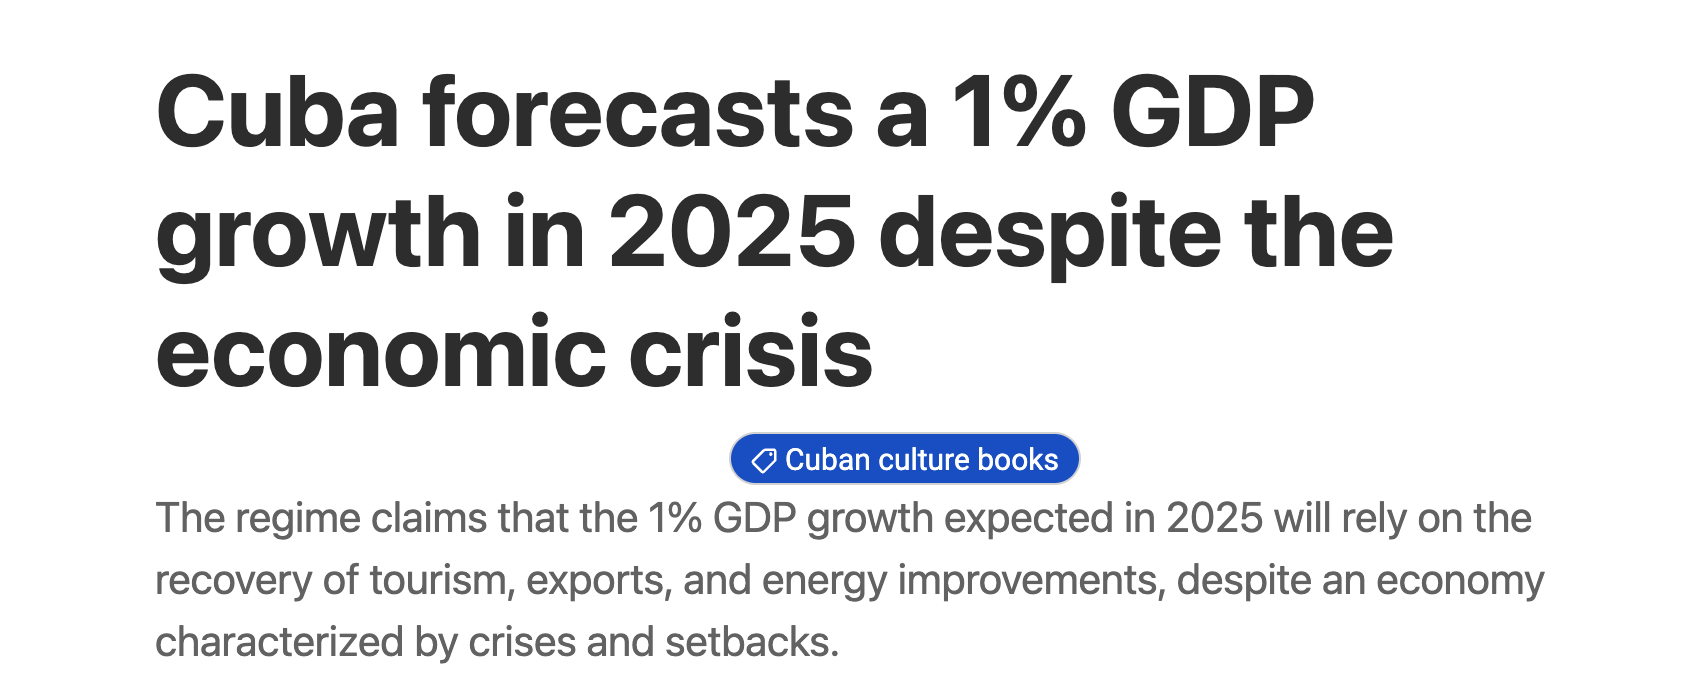
\includegraphics[width=0.8\textwidth]{/Users/chrisperez/Desktop/stat288-finalproject/images/news_1.png}} \\[1em]
  \fbox{
\includegraphics[width=0.8\textwidth]{/Users/chrisperez/Desktop/stat288-finalproject/images/news_3.png}}
\end{frame}

\begin{frame}{What's Really Happening in Cuba?}
  \centering
  \fbox{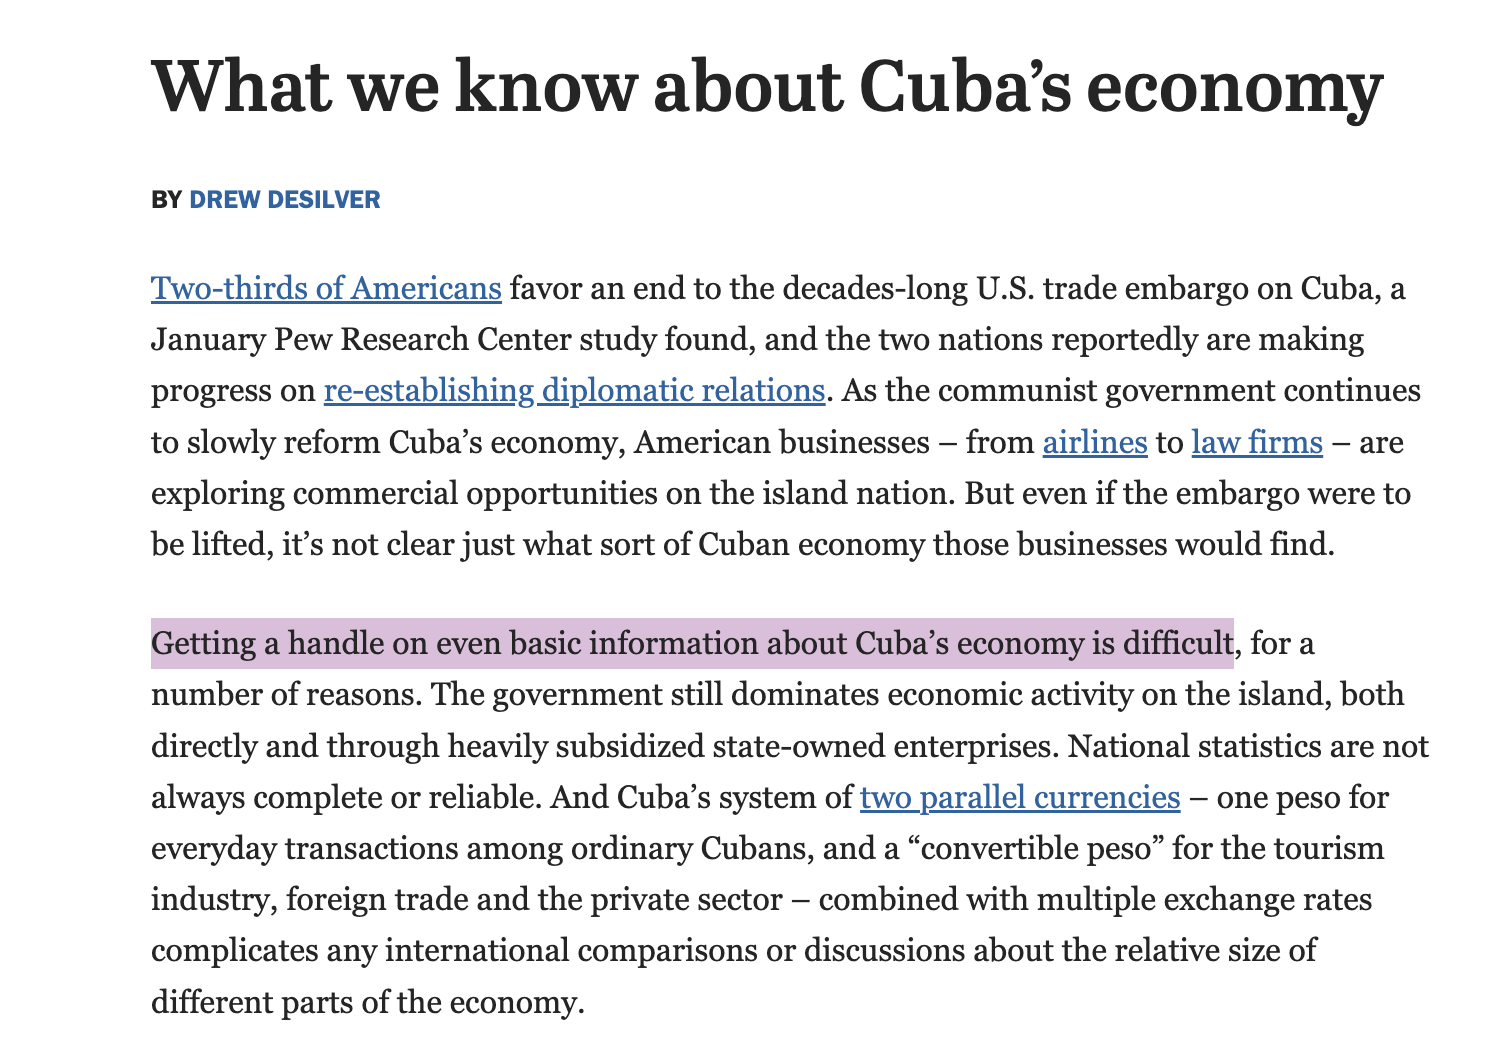
\includegraphics[width=0.8\textwidth]{/Users/chrisperez/Desktop/stat288-finalproject/images/news_4.png}}
\end{frame}


% MOTIVATION & CONTEXT
\begin{frame}{Motivation}
  \begin{itemize}
    \item Cuba's economic indicators are poorly reported or missing.
    \item International institutions lack consistent ground truth.
    \item Can satellite proxies and open data fill the gap?
  \end{itemize}
\end{frame}

  
\begin{frame}{Research Question}
  \begin{block}{Goal}
  Estimate spatial economic activity using observable data and a principled statistical model.
  \end{block}
  \pause
  \begin{itemize}
    \item Leverage nightlights, NDVI, and road density.
    \item Use Bayesian inference to estimate a latent variable $z_i$ per cell.
  \end{itemize}
  \end{frame}
  
% DATA SOURCES
\begin{frame}{Data Sources}
\begin{itemize}
    \item \textbf{Nighttime Lights (VIIRS)}: Urbanization and infrastructure.
    \item \textbf{NDVI}: Vegetation intensity.
  \item \textbf{Road Density}: Accessiblity and development.
\end{itemize}
\pause
All proxies standardized and aligned to 500m grid. Water masked. 2024.
\end{frame}

% MODEL OVERVIEW
\begin{frame}{Bayesian Latent Variable Model}
  \begin{itemize}
    \item Latent index $z_i$ per cell, measuring economic activity.
    \item Observation: $x_{i,k} \sim \mathcal{N}(\beta_k z_i, \sigma_k^2)$.
    \item Fixed $\beta_{\text{lights}} = 1$ for identifiability.
    \item Spatial smoothing via ICAR prior.
  \end{itemize}
  \end{frame}
  
\begin{frame}{Bayesian Latent Variable Model}
\centering

\includegraphics[width=0.8\textwidth]{/Users/chrisperez/Desktop/stat288-finalproject/images/plate.png}
\end{frame}

% POSTERIOR RESULTS
\begin{frame}{Posterior Results: Cuba (15km Grid)}
  \centering
  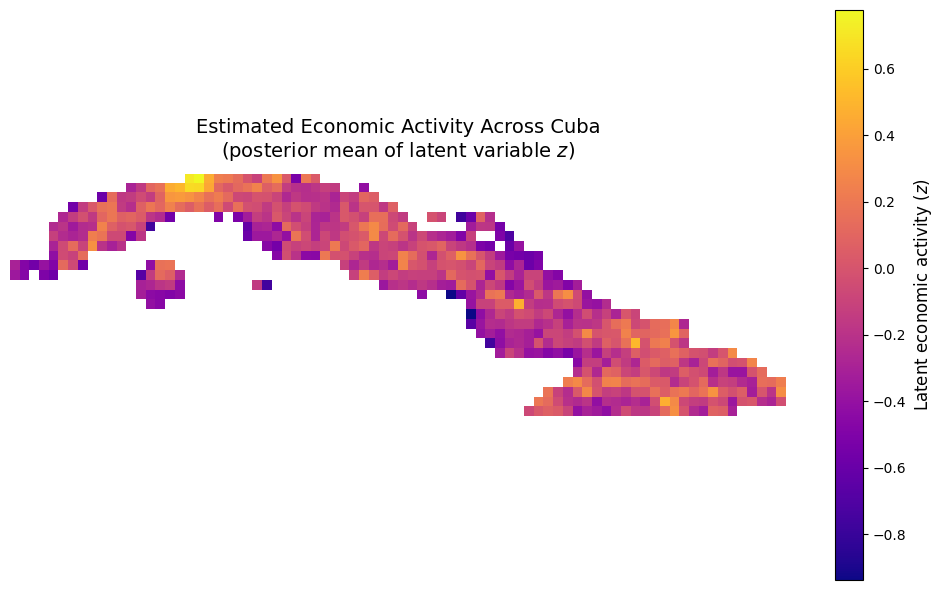
\includegraphics[width=0.7\textwidth]{/Users/chrisperez/Desktop/stat288-finalproject/images/fig1.png}
  \begin{itemize}
    \item High activity in Havana and other urban centers.
    \item Sparse regions have low $z$.
  \end{itemize}
\end{frame}

\begin{frame}{Posterior Uncertainty}
\centering
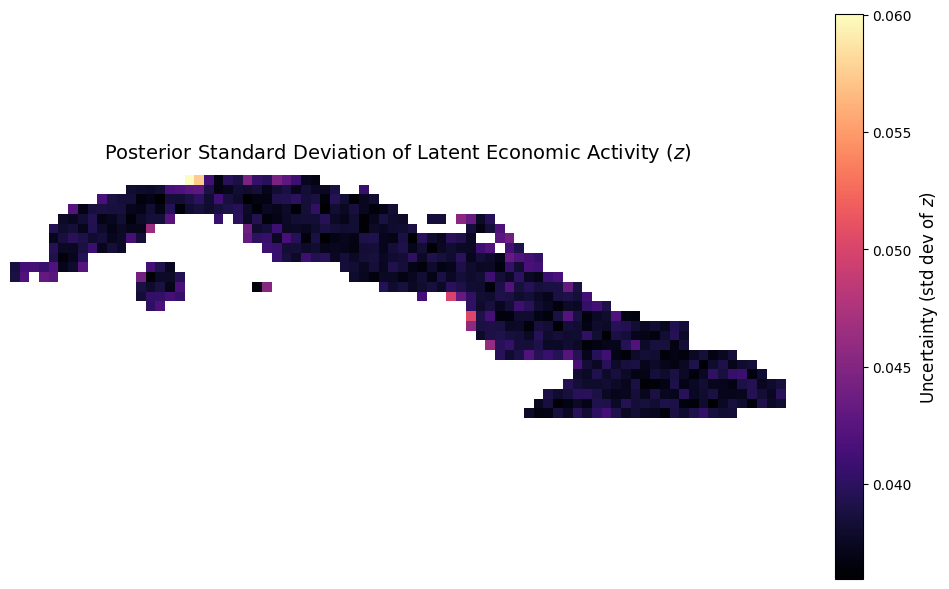
\includegraphics[width=0.6\textwidth]{/Users/chrisperez/Desktop/stat288-finalproject/images/fig2.png}
\begin{itemize}
  \item Posterior standard deviation is low ($\approx$ 0.04--0.06)
  \item Higher uncertainty in urban areas like Havana
\end{itemize}

\end{frame}

% COEFFICIENTS & DIAGNOSTICS
\begin{frame}{Model Coefficients}
\centering
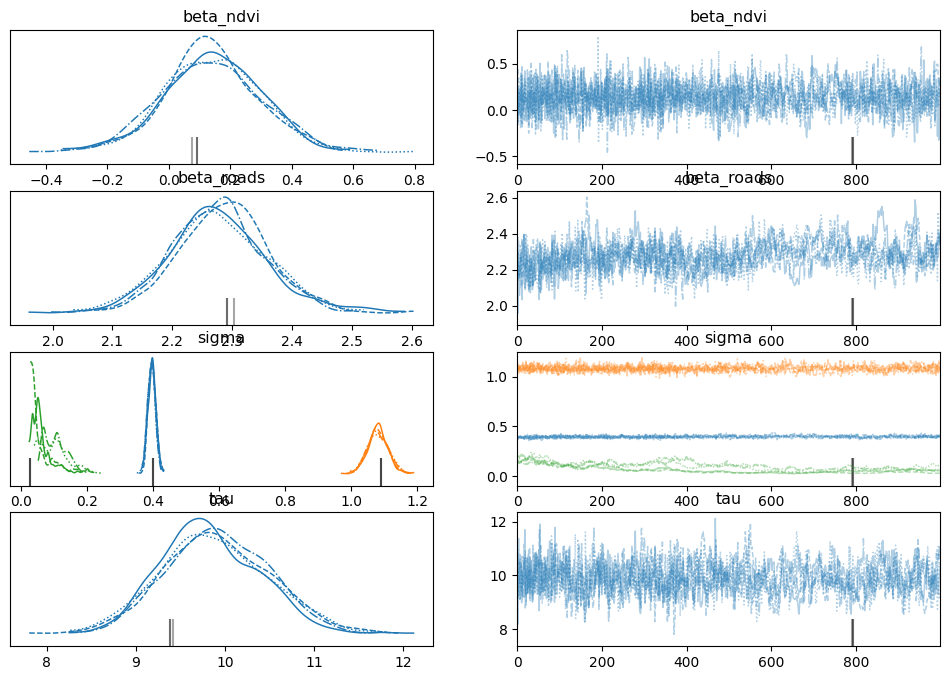
\includegraphics[width=0.7\textwidth]{/Users/chrisperez/Desktop/stat288-finalproject/images/fig_3_post_diagnostics.png}
\begin{itemize}
  \item $\beta_{\text{NDVI}} \approx 0.14$ (weakly positive).
  \item $\beta_{\text{roads}} \approx 2.29$ (strong positive).
  \item $\sigma$ values show road is low-noise; NDVI is high-noise.
\end{itemize}
\end{frame}

% MULTI-RESOLUTION
\begin{frame}{Multi-Resolution Overview}
  \begin{itemize}
    \item Question: How does resolution affect our estimates?
    \item Fit model at 5km, 10km, 20km blocks.
    \item Compare variance, posterior uncertainty, and coefficients.
  \end{itemize}
  \end{frame}
  
\begin{frame}{Resolution Comparison: Maps}
    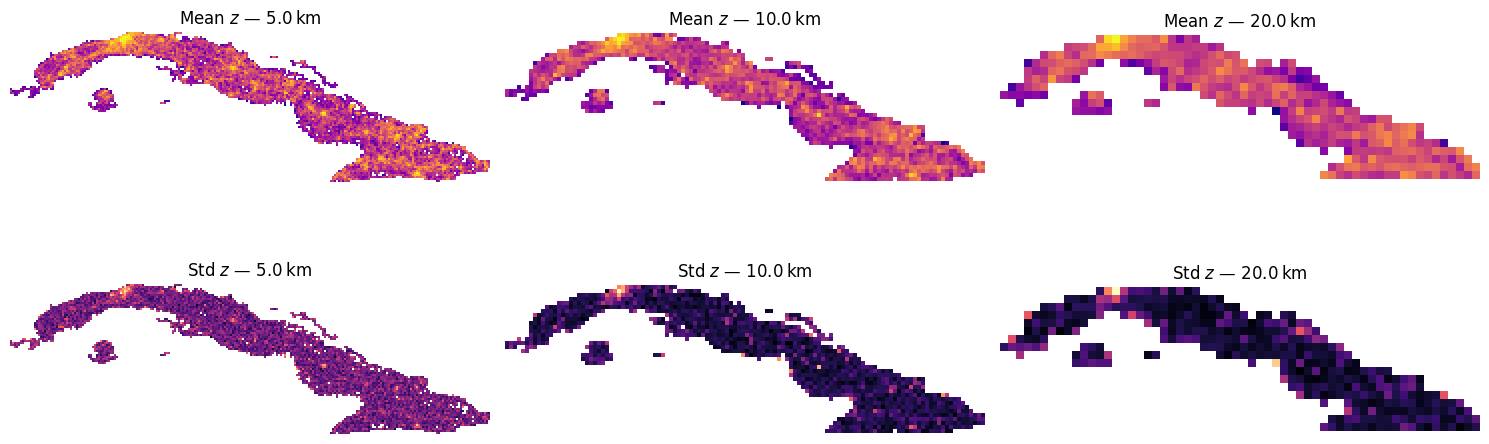
\includegraphics[width=\textwidth]{/Users/chrisperez/Desktop/stat288-finalproject/images/multires_cuba.png}
\end{frame}


\begin{frame}{Resolution Comparison: Trace Plots}
    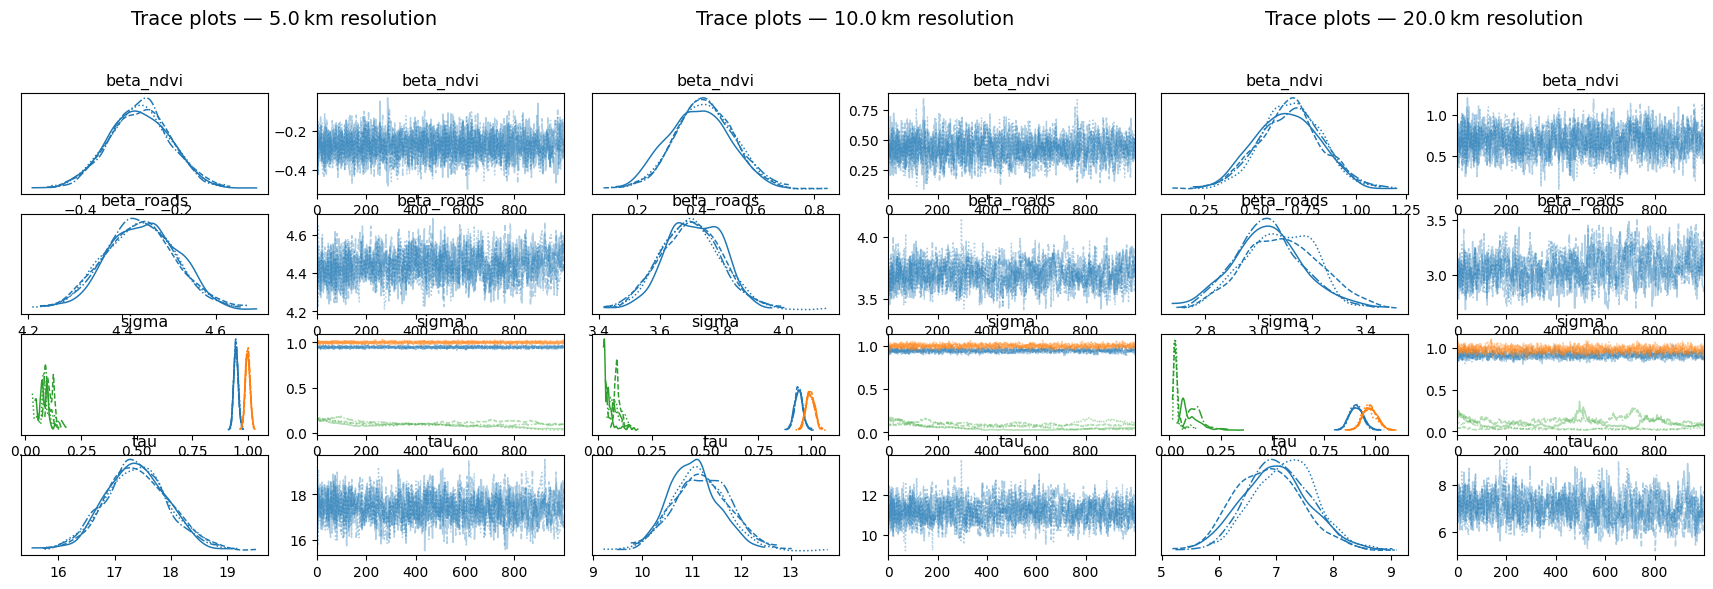
\includegraphics[width=\textwidth]{/Users/chrisperez/Desktop/stat288-finalproject/images/combined_trace_plots.png}
\end{frame}


  \begin{frame}{Multi-Resolution Results Summary}
    \begin{itemize}
      \item $\beta_{\text{NDVI}}$ flips from negative to positive as resolution increases
      \item $\beta_{\text{roads}}$ declines: 4.44 \textrightarrow{} 3.06
      \item Posterior variance in $z$ increases with block size
      \item Larger blocks allow more deviation between neighboring cells (smaller $\tau$)
    \end{itemize}
    \end{frame}
    
    

\begin{frame}{Zoom-In: Greater Havana and Camagüey}
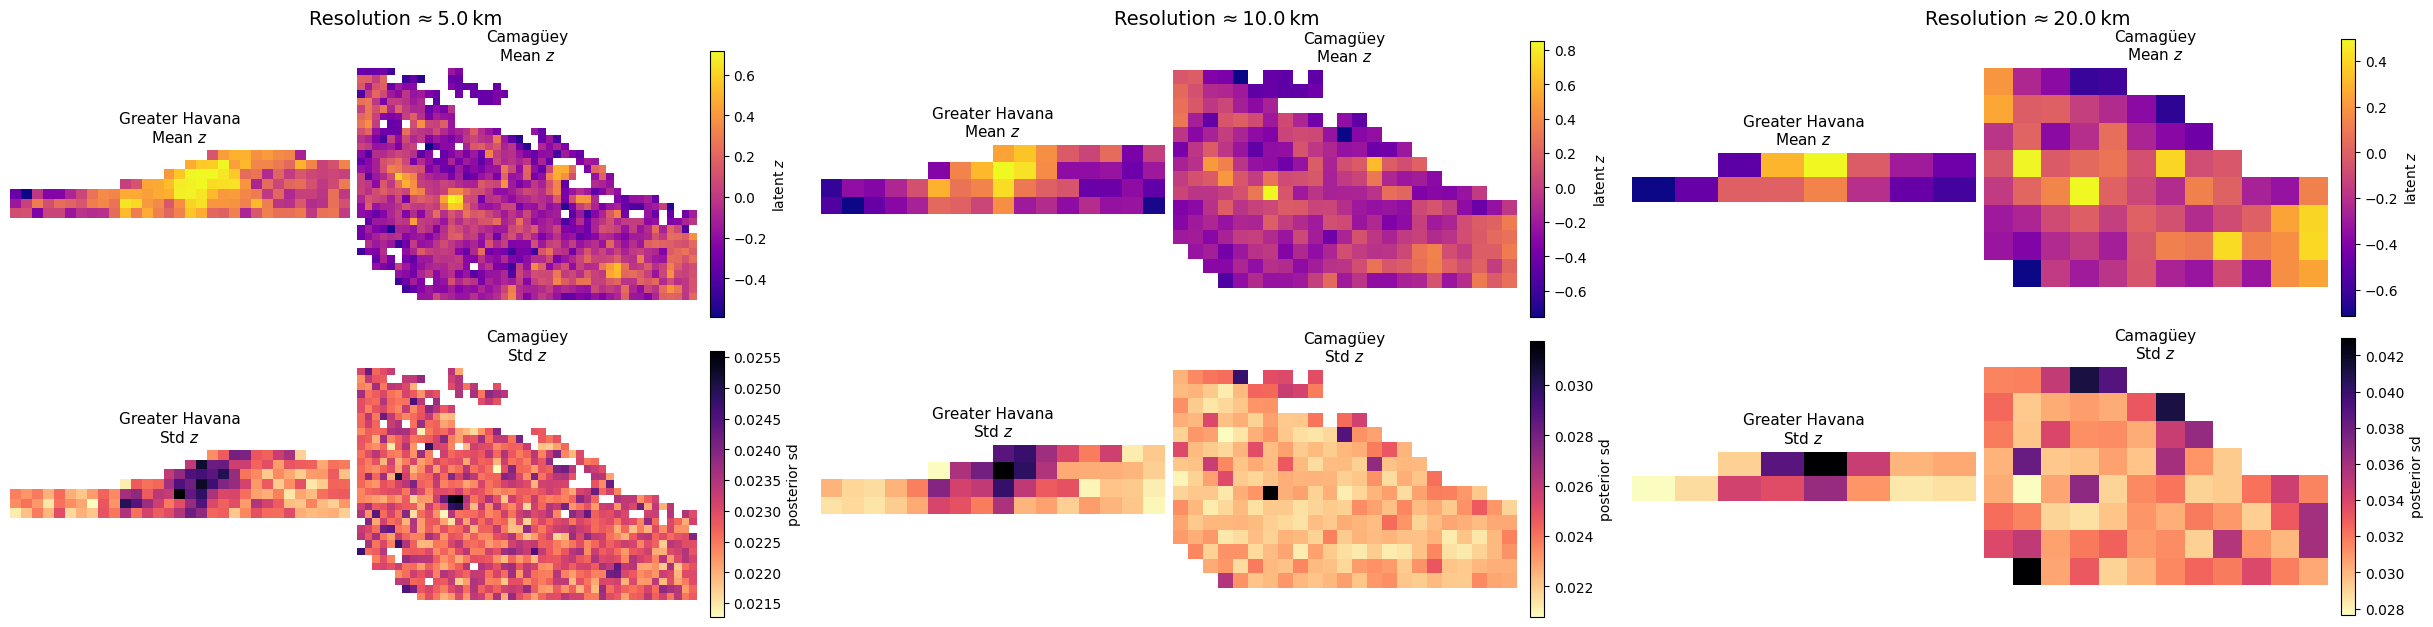
\includegraphics[width=\textwidth]{/Users/chrisperez/Desktop/stat288-finalproject/images/combined_maps.png}
\begin{itemize}
  \item Coarser resolution increases uncertainty per cell
  \item Urban vs. rural differences emerge clearly
\end{itemize}
\end{frame}


% CONCLUSION
\begin{frame}{Conclusion and Future Work}
  \begin{itemize}
    \item Satellite proxies capture meaningful patterns in $z_i$.
    \item Bayesian model provides uncertainty quantification.
    \item Immediate Next Step: Cross-validate approach on Dominican Republic.
    \item Future: Add time dynamics and explore spatially varying $\beta_k$.
  \end{itemize}
  \end{frame}
  
% thank you slide
\begin{frame}{Thank You!}
  \centering
  \Large
  Thank you! 
  Questions? Feedback?
\end{frame}

% REFERENCES
\begin{frame}{References}
  \begin{itemize}
    \item Liu, Bo et al. (2020). "An Economic Development Evaluation Based on the OpenStreetMap Road Network Density: The Case Study of 85 Cities in China." \textit{ISPRS Int. J. Geo-Inf.}, 9(9), 517. \href{https://www.mdpi.com/2220-9964/9/9/517}{https://www.mdpi.com/2220-9964/9/9/517}
    \item Steele, Jessica E. et al. (2017). "Mapping Poverty Using Mobile Phone and Satellite Data." \textit{J. Royal Soc. Interface}, 14(127), 20160690. \href{https://www.ncbi.nlm.nih.gov/pmc/articles/PMC5332562/}{https://www.ncbi.nlm.nih.gov/pmc/articles/PMC5332562/}
    \item Besag, J., York, J., \& Mollié, A. (1991). "Bayesian image restoration, with two applications in spatial statistics." \textit{Annals of the Institute of Statistical Mathematics}, 43(1), 1-20. \href{https://doi.org/10.1007/BF00116466}{https://doi.org/10.1007/BF00116466}
  \end{itemize}
  \end{frame}

\end{document}
